\section{Fresnel Zones}\label{sec:fresnel}
Taking into account that the application at hand involves radio communication it is important to talk about the Fresnel zones. The Fresnel zone is a long ellipsoid that stretches between the two antennas. Thus, it can be seen in Figure \ref{fig:fresnel_zones} the three Fresnel zones on the transmission path between A and B. 

\begin{figure}[h]
	\centering
	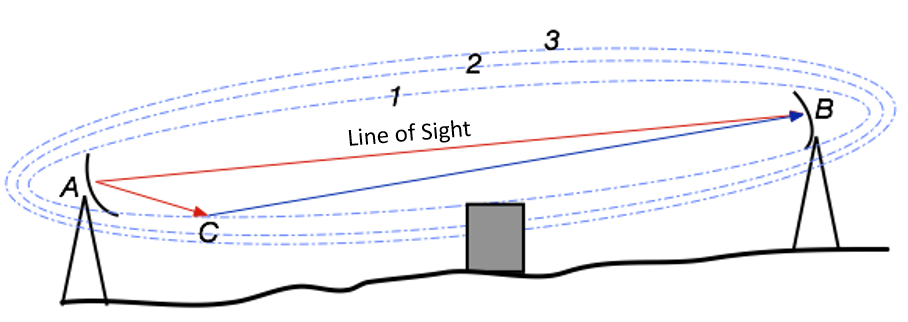
\includegraphics[scale=0.65]{figures/fresnel_zones.png}
	\caption{Fresnel zones between transmitter and receiver}
	\label{fig:fresnel_zones}
\end{figure}

%These Radio frequency line of sight is defined by Fresnel Zones which are ellipse shaped areas between two radios. The primary Fresnel zone is required to be at least 60$\%$ clear of any obstruction to ensure the highest performance of wireless link. 

The 1st zone is the ellipse with chords 1/2 wavelength longer than the direct path (ACB)

%If a reflective object is very near the direct path, the signal will experience a 180$^o$ phase shift and cancel the direct wave at the receiver.
%
%If a reflective object is tangent to the 1st zone, the electromagnetic wave will be shifted 180$^o$ because of the increased path length, undergo an additional 180$^o$ phase shift due to the reflection, and reinforce the direct wave at the receiver. Consequently, there should be no reflective objects in the 1st Fresnel zone.
%
%If unobstructed, radio waves will travel in a straight line from the transmitter to the receiver. But if there are reflective surfaces along the path, such as bodies of water or smooth terrain, the radio waves reflecting off those surfaces may arrive either out of phase or in phase with the signals that travel directly to the receiver. Waves that reflect off of surfaces within an even Fresnel zone are out of phase with the direct-path wave and reduce the power of the received signal. Waves that reflect off of surfaces within an odd Fresnel zone are in phase with the direct-path wave and can enhance the power of the received signal. Sometimes this results in the counter-intuitive finding that reducing the height of an antenna increases the signal-to-noise ratio.
%
%Fresnel provided a means to calculate where the zones are—where a given obstacle will cause mostly in phase or mostly out of phase reflections between the transmitter and the receiver. Obstacles in the first Fresnel zone will create signals with a path-length phase shift of 0 to 180 degrees, in the second zone they will be 180 to 360 degrees out of phase, and so on. Even numbered zones have the maximum phase cancelling effect and odd numbered zones may actually add to the signal power.[1]
%To maximize receiver strength, one needs to minimize the effect of obstruction loss by removing obstacles from the radio frequency line of sight (RF LoS). The strongest signals are on the direct line between transmitter and receiver and always lie in the first Fresnel zone.


! ! ! ! \url{https://en.wikipedia.org/wiki/Fresnel_zone}  ! ! ! !